\section{Introduction and background information}

This project is created with the minds of combining string arts, and pendulum; exploring the creative side of combining mathematics and physics. The project is themed under the subject ESC774: Into the real world oscillation. The research question is
\begin{quote}
    \emph{Is it possible to create any arbitrary image from pendulum art?}
\end{quote}
Or, in another way,
\begin{quote}
    \emph{Can an image be decomposed into multiple pendulum swings?}
\end{quote}

The research question is almost impossible to tackle with the pendulum that's affected by air resistance and the Coriolis force which gives the pendulum art their characteristics. Therefore, this paper scopes ourselves to a pendulum that's not subjected to any outer forces but gravity. We also allow a degree of freedom that the amount of paint that's dispensed per unit time is controllable

Because of these constraints, the only shapes that a pendulum can trace out are ellipses with varying sizes and rotation angles. It's then possible to reverse engineer these ellipses to figure out the initial condition of the pendulum.

The code that's written will be able to tell how to decompose an image into multiple ellipses, and the output contains
\begin{enumerate}[noitemsep]
    \item The ellipses that are used to create the image
    \item The brightness/darkness of each ellipse
\end{enumerate}
The final image will also then be plotted as a heatmap.

Since every ellipse can be traced back to a pendulum, we shall only focus on the ellipses for the rest of the paper. We shall give the ellipses only four degrees of freedom:
\begin{enumerate}[noitemsep]
    \item Semi-major axis length
    \item Semi-minor axis length
    \item Ellipse rotation
    \item Ellipse position
\end{enumerate}
It should be immediately obvious that the time-complexity for this algorithm is at minimum, $\mathcal{O}(n^4)$.

\section{Fourier transform and vector spaces}

The Fourier transform is a well-known procedure for decomposing any waves into sum of sine waves, which is commonly seen in audio programs, as shown in \cref{fig:audiogram}. That is, it maps the amplitude domain into the frequencies domain.
\begin{figure}[ht]
    \centering
    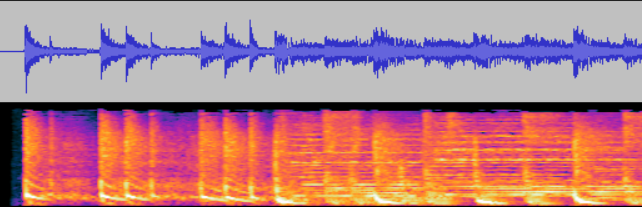
\includegraphics{spectrogramrickroll.png}
    \caption{The waveform and spectrogram view of the first few seconds of audio from the song Never Gonna Give You Up by Rick Astley}
    \label{fig:audiogram}
\end{figure}

In quantum mechanics, everything is represented as state vectors. A state vector must contain all the information about a system. In this mindset, the Fourier transform can be thought of a transformation of a vector $\ket{\psi}$ from the amplitude space to the frequencies space. Because no information is lost with the transform, the Fourier transform can be thought of a change of basis vector from the amplitude basis to the frequencies basis.

The Fourier transform naturally occurs when the momentum basis $\{\ket{p\prime}\}$ is projected onto the position basis $\{\ket{x\prime}\}$,
\begin{equation}
    \braket{x\prime}{p\prime} = \frac{1}{\sqrt{2\cpi\hbar}}\exp[\frac{\iu}{\hbar}x\prime p\prime].
\end{equation}
Thus, the Fourier transform is considered to be the special case where the basis conversion is between amplitude and frequencies. Generally, one can select or construct a basis to transform by themselves. In this paper, the problem will be tackled by using the transformation from the ellipses basis and the pixels basis by constructing the basis ourselves. Because the transform is going to be done using numerical methods, the basis constructed must be discretized.

\section{Construction of the image vector and the basis used}

We start from the construction of the image vector that we want to transform into the ellipse basis. This vector $\vv{B}$ will be in the pixels space.

The pixels basis can be easily constructed. For any picture of size $2n + 1$, we construct a grid as shown in \cref{fig:pixelsgrid} where each lattice point represents a pixel that will be plotted as heatmaps in the final image.
\begin{figure}
    \centering
    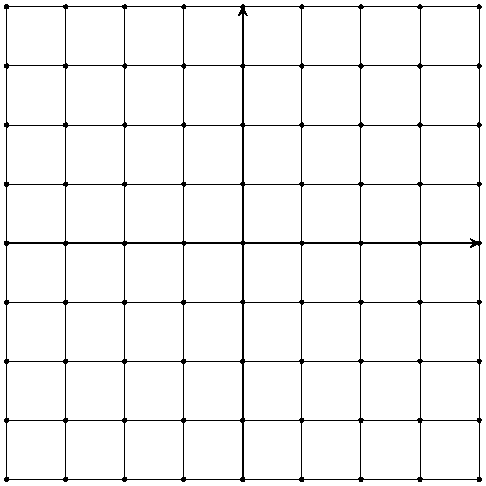
\includegraphics{pixelsmapping.pdf}
    \caption{Examples of pixels mapping where $n = 4$, and the grid size equals $2n + 1$}
    \label{fig:pixelsgrid}
\end{figure}

The mapping function $\mathcal{M}$ from cartesian coordinate centered at $(0, 0)$ to the pixel space can be written as
\begin{equation}
    \mathcal{M}(n, x, y) = x + n + 1 - (2n + 1)(y - n).
\end{equation}

Each pixel $b_n$ will then be assigned its value according to the brightness ranging from $0$ to $1$ where $1$ is the brightest. The whole picture can then be expressed as a column vector $\vv{B}$ containing the brightness value of each points. For an arbitrary $n$, the column vector will have the dimension $2n + 1$ which is called $N$:
\begin{equation}
    \vv{B} = \mqty[b_1 \\ b_2 \\ \vdots \\ b_{N - 1} \\ b_{N}].
\end{equation}

Now, we shall consider the ellipses that's drawn by the program to use as a basis. The ellipses are generated by the well-knowned midpoint ellipse algorithm which takes in $a$, the semimajor axis, $b$, the semiminor axis and outputs a tuple filled with the integers coordinates that that ellipse passes. The rotated ellipses also has to be in the set of basis; thus, we use a rotation matrix in two-dimensions;
\begin{equation}
    R(\theta) = \mqty[\cos\theta & \sin\theta \\ -\sin\theta & \cos\theta],
\end{equation}
and iterate $\theta$ from $0$ to $\flatfrac{\pi}{2}$.

Though, this method of generating rotated ellipses falls short for large ellipses because rounding points accuracy. There is some discontinuities in the rotated ellipses, but for the sake of the first prototype, this suffices already.

Each basis ellipses $e_1$,